\section{Design \& Konzept}
\label{sec:design-und-konzept}
In diesem Kapitel ...

\subsubsection{Framework}
Warum Framwork? Besonderheiten...
\subsection{Übersicht der Komponenten im Klassendiagramm}
\begin{sidewaysfigure}
		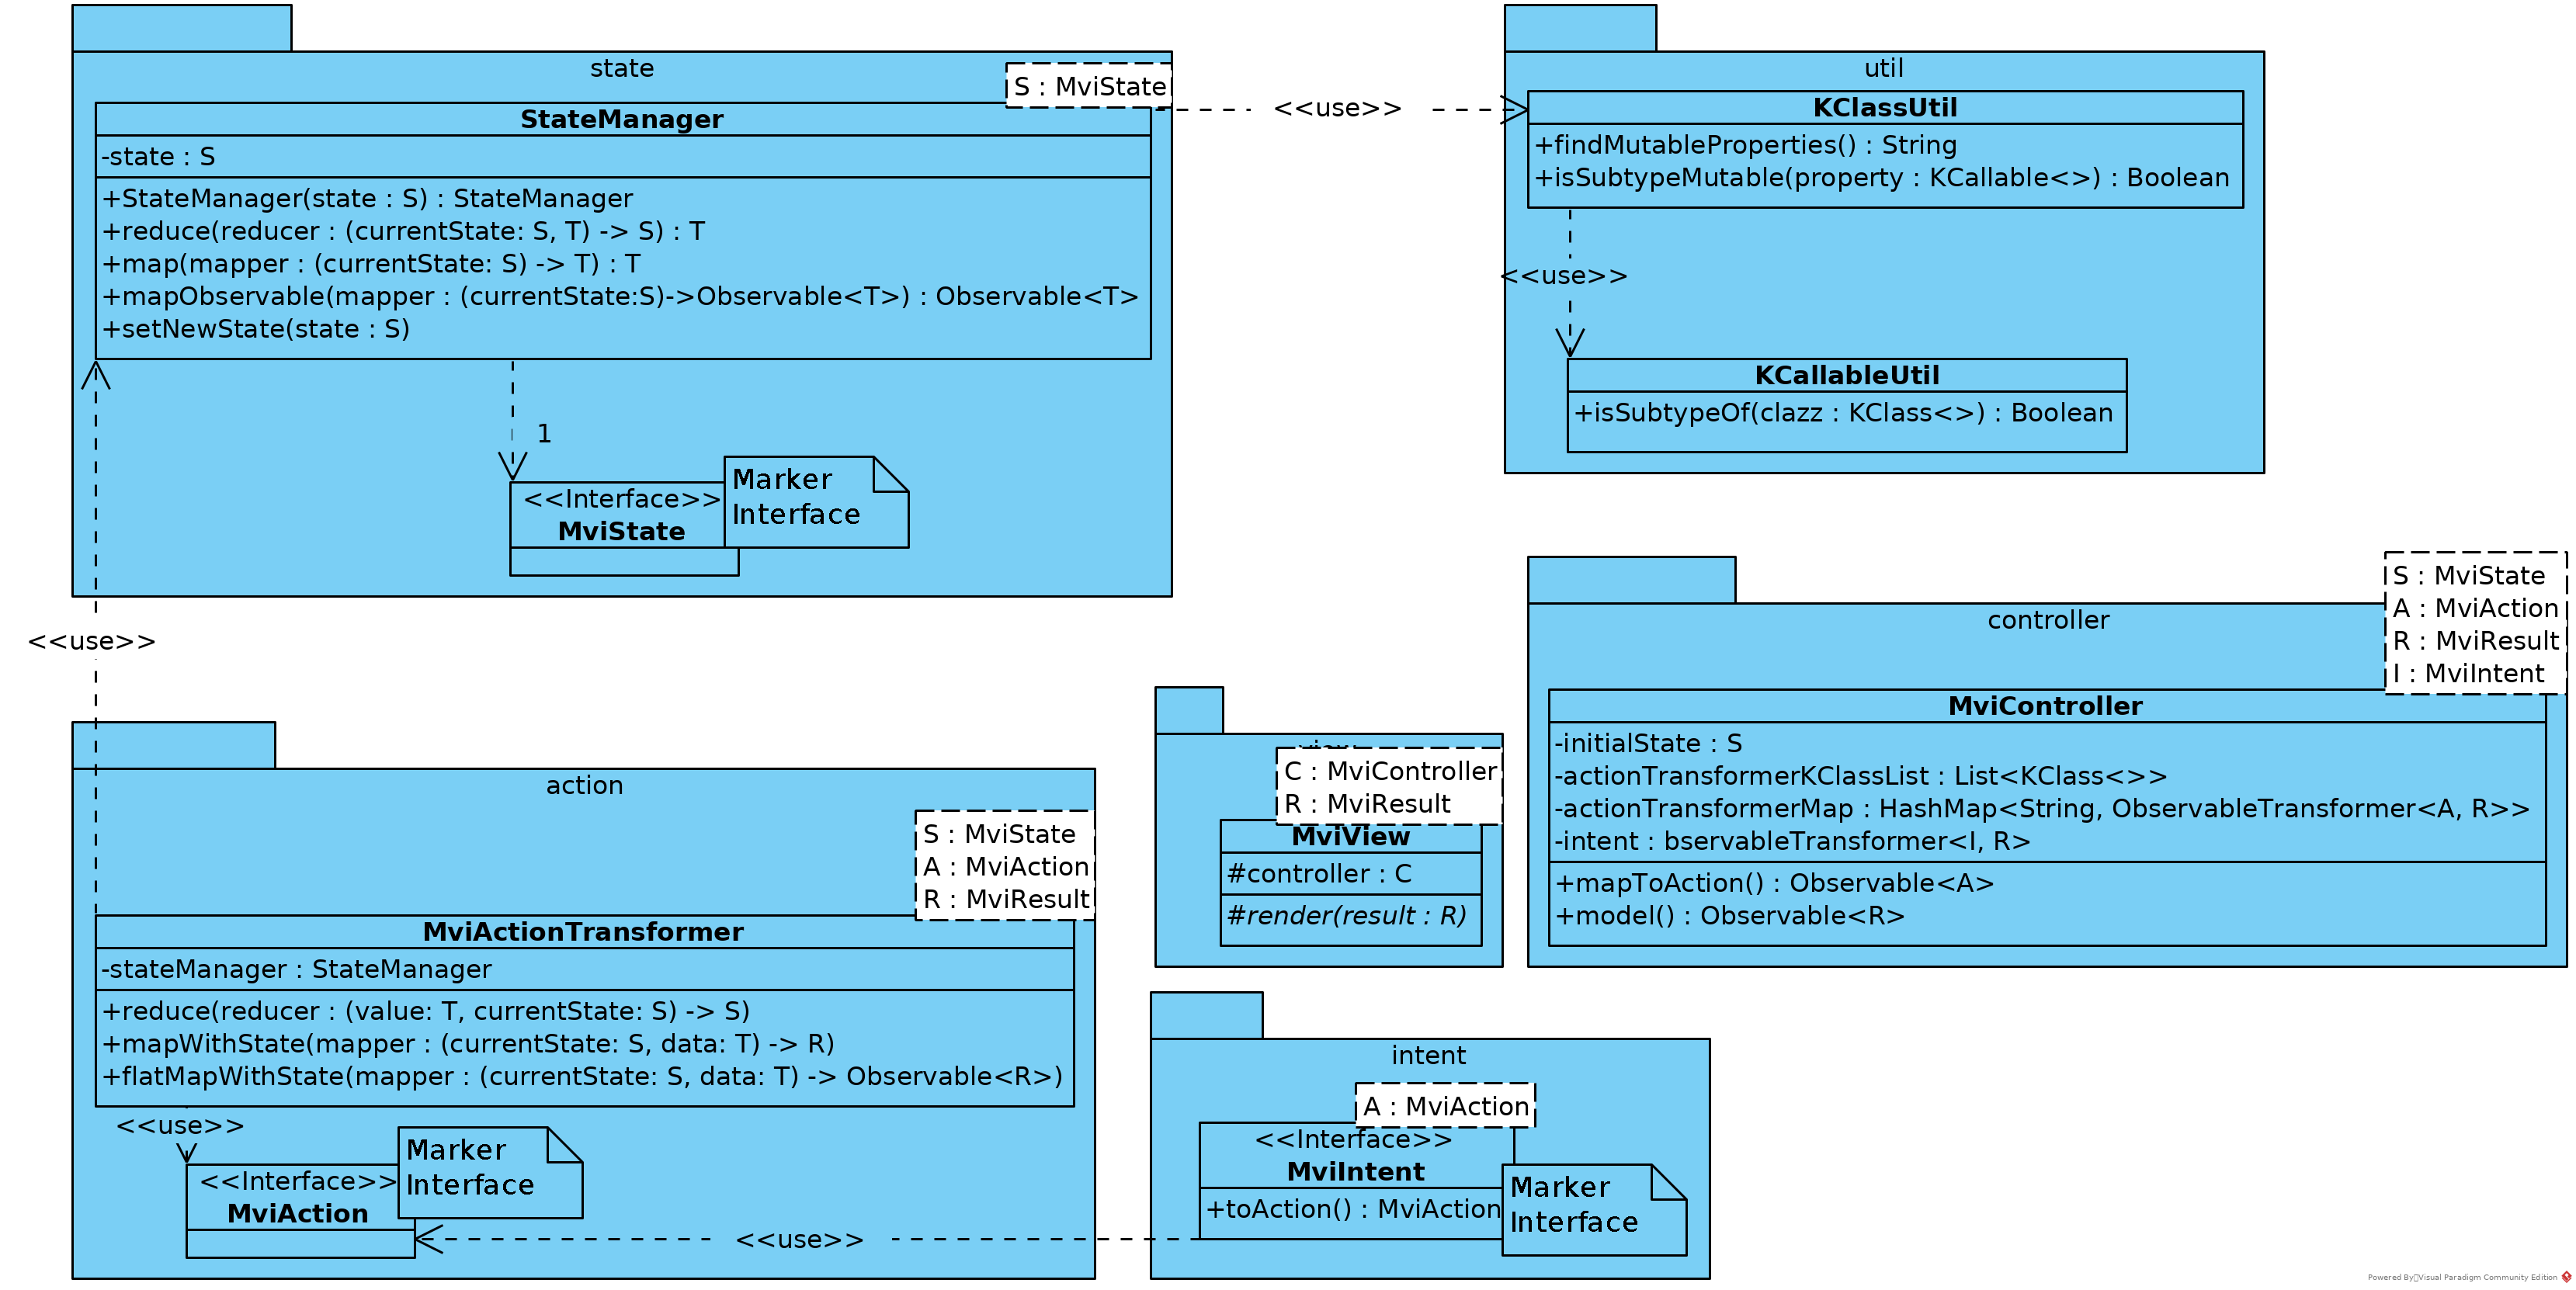
\includegraphics[width=\textwidth]{./images/framework-class-diagram}
		\caption{Komponenten im Klassendiagramm}
\end{sidewaysfigure}
\clearpage
\subsection{Zustand (State) und seine Verwaltung}
\label{subsec:zustand-und-statemanager}
In den Ausführungen von MVI wird der Zustand als eine Anhäufung von Werten betrachtet. Es bildet den Kern von MVI und muss im Normalfall vom Entwickler selbst verwaltet werden. Unter anderem muss garantiert sein, dass ein Zugriff und eine Modifikation des Zustands nur an einer Stelle erfolgen kann. Im Rahmen des Framworks wird eine Komponente genutzt, die diese Aufgaben für den Entwickler übernimmt und den Zustand 'managed': Der 'StateManager'.
\\\\
Dieser erwartet den initialen Zustand, der vom Entwickler an das Framework übergeben wird. Der Zustand wird dabei als generischer Parameter definiert und muss dem Interface 'MviState' entsprechen. Die Variable 'state' selbst ist eine der wenigen, die eine Mutation zulassen muss, wie später deutlich wird.
\\
Nachdem der Zustand überreicht wurde, wird geprüft, inwieweit dieser der Anforderung der Unveränderlichkeit entspricht. Sollte diese nicht gegeben sein, so wird eine Fehlermeldung ausgegeben und der Prozess gestoppt.
\\\\
Ist dies erfolgreich, so wartet der 'StateManager' mit Funktionalität auf, welche es ermöglicht einen neuen Zustand zu hinterlegen, sowie mit ihm sicher zu arbeiten. Ein neue Setzung des Wertes wird dabei durch die Kombinationen der Funktionen 'reduce' und 'setNewState' erreicht. 
\\\\
Erstere erwartet eine Funktion als Parameter, 'reducer', welche wiederum den derzeitigen Zustand übergeben bekommt. Diese wird aufgerufen und produziert einen neuen Zustand, der durch 'setNewState' als aktueller Zustand gesetzt wird. Dies geschieht allerdings nur unter der Prämisse, dass sich mindestens ein Wert innerhalb der Datenstruktur verändert hat.
\\
Als Zusatz stellt 'setNewState' sicher, dass es auch bei gleichzeitigen Zugriffen von mehreren 'Threads' zu keiner sogenannten unbeabsichtigten Wettlaufsituation (Race Condition) und damit inkonsistenten Daten kommt.
\\
An dieser Stelle wird erkennbar, weshalb die 'state' Variable zwingend veränderlich sein muss. Wäre diese nicht der Fall, so könnte ihr kein neuer Zustand zugewiesen werden.
\\\\
Die Methode 'map' nimmt genau wie 'reduce' eine Funktionen entgegen, welche den aktuellen Zustand erhält. In dieser kann der Entwickler auf die Attribute des Zustands zurückgreifen, jedoch keine neuen bestimmen.
\\\\
Diese Komponente ist nicht direkt für den Nutzer zugänglich und wir ausschließlich intern im Framework genutzt. Es verhindert, dass der Zustand an einer beliebigen und nicht vorgesehenen Stelle verändert werden kann.

\subsection{Intent, Action und Result}
\label{subsec:intent-action-und-result}
Die im Titel genannten Komponenten dienen der Übermittlung und Beschreibung von Informationen innerhalb des 'Kreislaufs' vom MVI. Diese müssen vom Entwickler selbst gestellt werden, erhalten dabei jedoch Vorgaben vom Framework.
\\\\
So muss zu jedem Intent eine Action existieren. Hierfür wartet das Framework mit dem Interface 'MviIntent' auf, das genanntes erzwingt und die Erfüllung dieser Anforderung sicherstellt. Realisiert wird dies durch die Funktion 'mapToAction', die der Entwickler später implementieren muss und eine 'Action' zurück gibt.  
\\\\
Ähnlich wie auf einen Intent eine Action erfolgt, zieht eine Action ein Result nach sich. Auch das gibt das Framework durch ein Interface namens 'MviAction' vor und muss vom Entwickler angewandt werden. Das Result findet seine Anwendung später in der View und wird ebenfalls mit einem Interface versehen.
\\
\\
Sämtliche der hier aufgeführten Strukturen sollten mit ihrem Namen die vorgesehene Intention signalisieren. Zusätzlich müssen sie in der Lage sein weitere Nutzdaten (Payload) aufzunehmen, die mit ihnen in Zusammenhang stehen und für den weiteren Verlauft Essential sind.

\subsection{Reaktiver unidirektionaler Datenfluss}
\label{subsec:reaktiver-unidirektionaler-datenfluss}
Für die Konzeptionierung der nächsten Komponenten gilt vorher zu klären, wie der geforderte reaktive unidirektionale Datenfluss in das Framework integriert werden soll. Dabei müssen Daten synchron oder asynchron verarbeitet und die Option zur Nebenläufigkeit (Concurrency) geboten werden. Zu diesem Zweck bedarf es einem Tool, welches das bereits aufgeführte 'Observer' und 'Iterator' Pattern nutzt. In diesem Zusammenhang taucht oft das Objekt 'Observable' auf, das genau diese Anforderungen erfüllt.  

\subsection{Transformer und die Business-Logik}
Ein elementaren Bestandsteil einer Anwendung macht die Businesslogik aus. Sie ist im Falle von MVI allein verantwortlich für das Abändern des Zustands und sollte strikt von anderen Komponenten getrennt sein.
Hierfür stellt das Framework den 'ActionTransformer zu Verfügung.
\\\\
Wie der Name vermuten lässt, ist die 'Action' unter anderem ausschlaggebend für die Nutzung der Komponente. Jeder 'Action' wird dabei ein 'ActionTransfomrer' zuteil, welcher über der ersten der zwei generischen Parameter, dem 'A', definiert wird. Dieser Parameter setzt voraus, dass das eingesetzte Objekt vom Interface 'MviAction' nutzen macht. Der zweite generische Parameter 'R' sieht ein Objekt vor, dass dem Interface 'MviResutlt' entstammt. Hier wird das zugehörige Result zur angegebenen Action eingefügt. 
\\\\
Der 'ActionTransformer' ermöglicht die Interaktion mit dem Zustand durch eine Variationen an Funktionen. Dafür benötigt er einen 'StateManager' welcher im bei seiner Erstellung übergeben werden muss. Die Funktionalität kann dabei - ähnlich wie beim 'StateManger' - in zwei Kategorien unterteilt werden:
\begin{enumerate}
	\item Die, in der ein neuer Zustand erzeugt wird und
	\item die, in der ausschließlich auf die Daten zugegriffen wird
\end{enumerate} 
Zu ersten Kategorie gehört lediglich die 'reduce' Methode, welche auf die gleichnamige Methode im 'StateManager' zugreift. Auch sie bekommt eine Funktion als Parameter, jedoch mit dem Unterschied, dass diese zusätzlich den derzeitigen Wert in Bearbeitung enthält. Dies kann beispielsweise ein Item sein, dass
von einem Intent an die Action weitergegeben wurde. Auf Basis dieser zwei Werte kann der Entwickler einen neuen Zustand bestimmen, welcher intern über den 'StateManager' gesetzt wird. Diese Operation findet auf der in Kapitel
\ref{subsec:reaktiver-unidirektionaler-datenfluss}
präsentierten 'Observable' Klasse statt und legt diese auch als Rückgabewert fest.
\\\\
In die zweite Kategorie fallen die Methoden 'mapWithState' und 'flatMapWithState', die beide die gleiche Funktion wie sie auch bei 'reduce' verwendet wird erhalten. Ihnen ist es nicht gestattet eine neuen Zustand herzustellen, sie können lediglich mit ihm arbeiten. Die 'flatMapWithState' Methode grenzt sich dadurch ab, das sie erlaubt andere asynchrone Funktionalität auszuführen, die ebenfalls einen Wert vom Typ 'Observable' zurückgibt und dabei Seiteneffekte berücksichtigt.
\\
Alle hier aufgezählten Methoden operieren auf den anfangs genannten generischen Parametern. 
\\\\
Somit ist im Quellcode klar ersichtlich, inwieweit eine Abänderung der Zustands gewollt ist und wann dieser lediglich mitsamt seiner Daten für den weiteren Verlauf benötigt wird. Hinzu kommt hier auch die automatische Handhabung von Seiteneffekten und asynchroner Funktionalität. Dies garantiert, dass der Zustand keine unabsichtliche Modifikation erfährt und zu jedem Zeitpunkt nur einer auf ihn zugreifen kann.

\subsection{Controller als Bindeglied}
Der Controller vereint die bisher beschriebenen Komponenten und 'kontrolliert' bzw. koordiniert anhand dieser den Aufruf der Business-Logik. Er stellt das Bindeglied zwischen der View, einer 'Action' und dem dazugehörigen 'ActionTransormer' dar und sorgt für den Aufruf von ebendiesem. 
\\\\
Dafür muss er über die vom Entwickler angedachte Form des Zustands, Intents, Action und Result informiert werden. Dies geschieht wie bei den vorherigen Komponenten durch die Angabe mehrerer generischer Parameter. Überdies erhält der Controller für seine Konstruktion den initialen Zustand und eine Liste von Namen der zugehörigen 'ActionTransformer' vom Entwickler.
\\\\
In der initialen Phase verifiziert der 'Controller', dass alle 'ActionTransformer' von der hinterlegten 'Action' und dem 'Result' abstammen um späteren Konflikten vorzubeugen. Anschließend wird der 'StateMananger' mit dem überlieferten Zustand instanziiert. Im letzten Schritt erzeugt der 'Controller' alle 'ActionTransformer' die jeweils einen 'StateManager' zugewiesen bekommen und speichert diese in Form von Schlüssel (Name des Transformers) und dazugehörigem 'ActionTransformer' in dem Attribut 'actionTransformerMap' ab.
\\\\
Im Controller selbst existieren zusätzlich zwei Funktionen und eine Variable, von denen nur letztere von außen Zugänglich ist: 'intent'. Sie stellt die in MVI beschriebene Intent-Funktion dar und dient als Einstieg in den unidirektionalen Kreislauf. Wird sie aufgerufen so führt sie die interne 'mapToAction' Methode aus, die mittels der im 'MviIntent' Interface definierten 'toAction' Methode, den 'Intent' in eine 'Action' umwandelt.
\\\\
Die zweite und zugleich auch letzte Funktion ist die 'model' Methode. Sie nimmt die 'Action', ermittelt ihren Klassenamen und entnimmt auf Grundlage dessen den entsprechenden 'ActionTransformer' aus der 'actionTransformerMap'. Die dort enthaltende Business Logik wird dann ausgeführt und das 'Result ', verpackt in einem 'Observable', nach 'oben' durchgereicht.
\subsection{View}
Die 'View' stellt den obersten Teil des Frameworks dar und besitzt im Kern zwei Eigenschaften: Sie reicht die 'Intents' an ihren 'Controller' weiter und verarbeitet das von ihm erhaltene 'Result'. Für beide werden erneut generische Parameter definiert. Einmal einer welcher aussagt, dass das eingefügte Objekt vom 'MviController' abstammen und ein zweiter, der dem 'MviResult' Interface entsprechen muss.
\\\\
Hierfür etabliert das Framework die 'MviView' Klasse, von der die 'View' abstammen muss. Sie stellt die oben geschilderten Anforderungen sicher, indem sie den Entwickler zwingt, ein Attribut zu hinterlegen und eine Funktionen zu implementieren. Bei ersterem handelt es sich um das Objekt, dass der Entwickler als 'MviController' ersonnen hat, bei letzterem um eine Methode, die ein 'Result' als Parameter erwartet. In dieser soll vom Entwickler die Logik stehen, welche für das aktualisieren des User Interface (UI) zuständig ist. 

\subsection{Anleitung zur korrekten Nutzung}
Um die Handhabung des Frameworks und die für den Entwickler vorgesehenen Komponenten besser nachzuvollziehen, wird im folgenden eine kurze Schritt für Schritt Anleitung dargelegt:
\begin{enumerate}
	\item Anlegen der Klasse für den Zustand im Verbund mit 'MviState'
	\item Anlegen sämtlicher Actions im Verbund mit 'MviAction
	\item Anlegen sämtlicher Intents im Verbund mit 'MviIntent' und obigen 'Actions'
	\item Anlegen sämtlicher Results im Verbund mit 'MviResult'
	\item Implementierung der Business Logik auf Basis der 'ActionTransformer' Klasse
	\item Implementierung des Controllers auf Basis der 'MviController' Klasse
	\item Implementierung der View auf Basis der 'MviView' Klasse
\end{enumerate}